\documentclass[12pt]{article}

\usepackage{sbc-template}

\usepackage{graphicx,url}

\usepackage[brazil]{babel}   
\usepackage[utf8x]{inputenc}  
\usepackage{minted}
\usepackage{listings}
\usepackage{hyperref}
     
\sloppy

\title{INF01121 - Modelos de linguagem de programação\\ Análise evolutiva da linguagem Java}

\author{Lucas Valandro da Rocha, Érico Monteggia de Moura}

\address{Instituto de Informática -- Universidade Federal do Rio Grande do Sul
  (UFRGS)\\
  Caixa Postal 15.064 -- 91.501-970 -- Porto Alegre -- RS -- Brasil
\email{lvrocha@inf.ufrgs.br, emmoura@inf.ufrgs.br}
}

\begin{document} 

\maketitle

\begin{abstract}
  Java is one of the most well known and popular programming languages in the modern programming landscape and boasts billions of devices running applications developed in Java. This article briefly analyzes the evolution of this language since version 8 up to version 11, highlighting defining features of each version, as well as the basic characteristics of the language itself.
\end{abstract}
     
\begin{resumo} 
  A linguagem de programação Java é uma das linguagens mais conhecidas e utilizadas no panorama moderno de programação e bilhões de dispositivos rodam aplicações desenvolvidas em Java. Este artigo faz uma breve análise da evolução desta linguagem desde a versão 8 até a versão 11, ressaltando funcionalidades marcantes adicionadas em cada versão, assim como uma análise de suas características básicas .
\end{resumo}


\section{Introdução}

É extremamente importante para um desenvolvedor se manter atualizado em relação às linguagens de programação e às ferramentas que o mesmo utiliza no seu dia a dia, uma vez que novas adições podem ampliar as possibilidades oferecidas e tornar seu fluxo de trabalho mais fácil e eficiente. 

Este artigo consiste na avaliação das principais funcionalidades que foram adicionadas nas versões mais recentes da linguagem Java, da versão oito (8) até a versão onze (11). Através de exemplos serão expostas - com base na opinião dos autores - as funcionalidades consideradas mais interessantes e que trazem mais vantagens para os desenvolvedores.

Adicionalmente, será feita uma análise resumida das características básicas da linguagem e como ela aplica conceitos de modelos de linguagem de programação, como simplicidade, ortogonalidade, portabilidade, entre outras.

\section{A linguagem Java} \label{sec:firstpage}

\cite{wikipediaJava} Java é uma linguagem de programação orientada a objetos desenvolvida na década de 90 por uma equipe de programadores chefiada por James Gosling, na empresa Sun Microsystems.

A linguagem Java foi inicialmente desenvolvida para ser utilizada em dispositivos móveis; entretanto, ganhou uma enorme força com o avanço meteórico da internet, no final da década de 90, através de tecnologias como \textit{Java Applets} e JSP (\textit{JavaServer Pages}) que permitiram que Java fosse usado facilmente em navegadores para internet. Desde seu lançamento, em maio de 1995, a plataforma Java foi adotada mais rapidamente do que qualquer outra linguagem de programação. 

\subsection{Características da linguagem}

\begin{itemize}
    \item \textbf{Simplicidade};
    \item \textbf{Orientação a objetos};
    \item \textbf{Portabilidade} - Independência de plataforma - \textit{"write once, run anywhere"};
    \item \textbf{Recursos de Rede} - Possui extensa biblioteca de rotinas que facilitam a cooperação com protocolos TCP/IP, como HTTP e FTP;
    \item \textbf{Segurança} - Pode executar programas via rede com restrições de execução.
\end{itemize}

\subsection{Java Virtual Machine}

Um dos fundamentos básicos da linguagem Java é a independência de plataforma. Um código em Java pode ser escrito uma vez, e executado em qualquer plataforma que suporte a linguagem, independente da arquitetura da máquina.

A linguagem é construída em cima de uma máquina virtual, a \textit{Java Virtual Machine} (JVM). Desta maneira, o código que o desenvolvedor Java escreve não é compilado para a arquitetura da máquina final, mas sim para um código intermediário .class (\textit{bytecode}). A JVM, por sua vez, traduz o código intermediário para código apropriado para a arquitetura alvo, dependendo da implementação da JVM para cada arquitetura e sistema operacional.

\begin{figure}[ht]
\centering
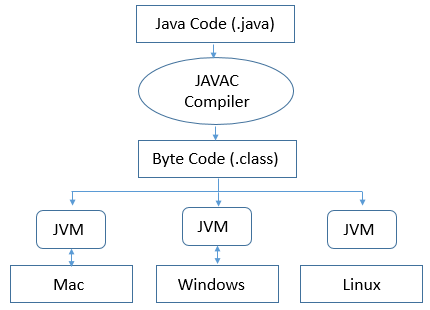
\includegraphics[width=.5\textwidth]{java-virtual-machine.png}
\caption{Fluxo de compilação de um programa em Java}
\label{fig:java-virtual-machine}
\end{figure}

\section{Java 8}

A versão, lançada em Março de 2014, foi considerada uma das versões com mudanças mais drásticas na linguagem, pois introduziu o paradigma funcional através de expressões lambda.

\subsection{Interfaces Funcionais}
\cite{functionalinterfaces} Functional Interfaces são todas as interfaces que possuem um método à ser implementados, ou em outras palavras, um método abstrato. Isso quer dizer que várias interfaces que já existiam e que atendiam a essa premissa, automaticamente se tornaram interfaces funcionais. O compilador consegue reconhecer essas interfaces e disponibilizá-las para o desenvolvedor trabalhar, por exemplo, com expressões lambdas.

\begin{minted}{java}
@FunctionalInterface
public interface Function<T, R> {
    ...
}
\end{minted}
\centerline{\textbf{Exemplo 1. Implementação \textit{Function} no pacote \textit{java.util.function}.}}
\hfill \break

A interface \textit{Function} é a forma mais simples e geral de expressar uma função lambda em Java. Ela é uma interface funcional em Java que recebe um parâmetro de entrada e retorna outro parâmetro qualquer.

\begin{minted}{java}
Function<Integer, String> intToString = Object::toString;
assertEquals("5", intToString.apply(5));

\end{minted}
\centerline{\textbf{Exemplo 2. Utilização da interface \textit{Function}.}}
\hfill \break

A criação de interfaces funcionais em Java criou uma série de possibilidades, e agregou diversos benefícios do paradigma funcional para a linguagem, como: legibilidade do código, facilidade de manipulação de dados e etc.

\subsection{Classe \textit{Optional}}

A classe \textit{Optional} foi introduzida na versão 8 do Java, e trouxe uma maneira totalmente nova de trabalhar com valores nulos dentro da linguagem, também permitindo maneiras de manipulação utilizando conceitos de programação funcional.

\begin{minted}{java}
Car ferrari = new Car();
if(ferrari.getColor() != null) {
    System.out.println("This " + ferrari.getColor() + 
        "Ferrari is awesome"); 
}
    
\end{minted}
\centerline{\textbf{Exemplo 3. Código sem a utilização de \textit{Optional}.}}
\hfill \break

Podemos observar que em versões mais antigas de Java, a forma de verificar se uma variável é nula era baseada em uma mesma referência, nesse caso, o objeto \textit{ferrari}. Com a utilização da classe \textit{Optional}, podemos reaproveitar a referência que foi utilizada para a verficação, para assim encadearmos com a chamada de algum outro método, nesse caso, o método \textit{ifPresent()}.

\begin{minted}{java}
Optional.ofNullable(ferrari.getColor())
        .ifPresent(color -> {
            System.out.println("This " + color
            + "Ferrari is awesome");
        });
\end{minted}
\centerline{\textbf{Exemplo 4. Código com a utilização de \textit{Optional}.}}

A classe \textit{Optional} provê uma facilidade na verificação de nulidade de uma variável, e também facilita a leitura do código através da reutilização da variável  como entrada do método \textit{ifPresent()}, ou quaisquer outros de seus métodos.


\section{Java 9}

A nona versão do Java foi lançada em setembro de 2017 e trouxe melhorias, e incrementos, nas interfaces funcionais que foram disponibilizadas na versão passada, juntamente com melhorias no algoritmo de \textit{garbage collection}.

\subsection{Métodos privados em interfaces}

\cite{quickGuide} A partir da nona versão de Java, é possível declarar métodos privados dentro de interfaces, o que retira a obrigatoriedade de todos os métodos de uma interface serem implementados, e também permite a escrita de um código mais isolado e reusável.

\begin{minted}{java}
public interface CarService {
    default long getNumberOfWhiteCars(List<Car> cars) {
        return cars.stream()
                   .filter(car -> car.getColor() == Color.WHITE)
                   .count();
    }
 
    default long getNumberOfRedItems(List<Car> cars) {
        return cars.stream()
                   .filter(car -> car.getColor() == Color.RED)
                   .count();
    }
}
\end{minted}

\centerline{\textbf{Exemplo 5. Código sem a utilização de métodos privados dentro de interfaces.}}

\begin{minted}{java}
public interface CarService {
    private long getNumberOfAvailableCars(List<Car> cars,
            Predicate<Item> filteringPredicate) {
                return cars.stream()
                        .filter(filteringPredicate)
                        .count();
    }
 
    default long getNumberOfWhiteCars(List<Car> cars) {
        return getNumberOfAvailableCars(cars, 
        car -> car.getColor() == Color.WHITE); 
    }
 
    default long getNumberOfRedCards(List<Car> cars) {
        return getNumberOfAvailableCars(cars,
        car -> car.getColor() == Color.RED);
    }
}
\end{minted}
\centerline{\textbf{Exemplo 6. Utilização de métodos privados para encapsular lógica compartilhada.}}

\subsection{Novos métodos para a classe \textit{Optional}}

A classe \textit{Optional} sofreu melhorias já na nona versão da linguagem Java, tendo recebido novos métodos, entre eles um muito requisitado pelo comunidade, o método \textit{ifPresentOrElse()}, que elimina totalmente a necessidade de uma estrutura \textit{if/else} tradicional.

\begin{minted}{java}
Optional<String> color = Optional.ofNullable(ferrari.getColor());
if (color.isPresent()) {
    System.out.println("This " + color.get() + 
            "Ferrari is awesome!");
} else {
    System.out.println("This Ferrari " + 
            "doesn't have a color yet.");
}
\end{minted}
\centerline{\textbf{Exemplo 7. Código sem a utilização do \textit{ifPresentOrElse()}.}}

\begin{minted}{java}
Optional.ofNullable(ferrari.getColor())
        .ifPresentOrElse(color -> {
            System.out.println("This " + color + 
            "Ferrari is awesome!"); 
        }, () -> {
            System.out.println("This Ferrari " + 
            "doesn't have a color yet.");
        });
        
\end{minted}
\centerline{\textbf{Exemplo 8. Código com a utilização do \textit{ifPresentOrElse()}.}}
\hfill \break


Através do novo método \textit{ifPresentOrElse()} pode-se implementar lógicas com desvios condicionais de maneira mais simples e legível.

\section{Java 10}

\cite{javaDocs} A décima versão de Java foi lançada em março de 2018, não contendo grandes alterações ou criações de novas APIs; entretanto, houveram melhorias significativas para execução do Java 10 em \textit{containers} de \textit{Docker}.

\subsection{Declaração de variáveis sem tipo explícito}

Na versão 10 da linguagem Java é possível omitir o tipo de uma variável, deixando essa função para o compilador que pode facilmente realizar o trabalho.

\begin{minted}{java}
List<CarWithTwoDoors> car = Arrays.asList(new CarWithTwoDoors());
var car = Arrays.asList(new CarWithTwoDoors());
\end{minted}
\centerline{\textbf{Exemplo 9: Utilização da palavra reservada \textit{var}.}}
\hfill \break

Essa funcionalidade permite com que se escreva menos código duplicado, tornando o código menos verboso.

\subsection{Compilador \textit{Just-In-Time} experimental}
\cite{javajit} JIT compilation is a form of dynamic compilation which combines the use of Ahead-Of-Time (AOT) compilation and interpretation, and thus has advantages and disadvantages from both technologies.

\section{Java 11}

\cite{javaDocs} A décima primeira versão de Java foi lançada em setembro de 2018. Como destaque temos melhorias, e experimentos, nos algoritmos de \textit{garbage collection}, adição de mecanismos de criptografia nativos e outras melhorias nos pacotes de internet da linguagem (.net).

\subsection{Expressões lambda como variáveis locais}

A versão onze do Java introduziu a possibilidade de criação de variáveis locais utilizando expressões lambdas. Anteriormente apenas eram permitidas expressões lambdas em atributos da classe.

\begin{minted}{java}
public Integer getCarConsumption(Car car) {
    final Integer km = 120;
    IntFunction<Integer> averageConsumption = 
        (Car c) -> km * c.getConsuption();
    return averageConsumption.apply(car);
}
\end{minted}
\centerline{\textbf{Exemplo 10. Variável local contendo uma expressão lambda.}}
\hfill \break

\subsection{Monitoramento do Heap com baixo consumo}
\cite{javaDocs} Fornece uma maneira com baixa custo de energia para obter informações das alocações do Java Heap. Isso faz com que esse processo possa ser habilitado como padrão pela JVM, e também é possível obter informações sobre os objetos alocados ou não.


\section{Análise Crítica}
Nesta seção será feita uma análise da linguagem Java do ponto de vista da disciplina de modelos de linguagens de programação e seus conceitos. A análise será feita para cada conceito isoladamente.

\subsection{Simplicidade}
O conceito de simplicidade se refere aos comandos, operadores e estruturas da linguagem. Neste quesito, Java deixa muito a desejar, pois apresenta grande variedade e ambiguidade sintática e semântica. Por exemplo, um número inteiro pode ser incrementado de pelo menos quatro maneiras diferentes (\textit{a++}, \textit{a=a+1}, \textit{a+=1} e \textit{++a}) e o operador \textit{+} pode ser usado tanto para somar números quanto para concatenar \textit{Strings}.

\subsection{Ortogonalidade}
Ortogonalidade é a capacidade de combinar componentes básicos da linguagem. Estes devem ser independentes para que sua combinação tenha resultado previsível e não tenha efeitos colaterais. De maneira geral, Java segue bem este conceito, mas em alguns casos deixa a desejar, como no caso do operador \textit{+} que não permite o uso com elementos do tipo \textit{byte}.

\subsection{Expressividade}
Uma linguagem expressiva é capaz de descrever algoritmos de maneira facilmente inteligível tanto para o computador quanto para o ser humano. Java é uma linguagem bastante expressiva, devido em boa parte a sua forte orientação a objetos e a sua proximidade ao mundo real. Mesmo assim, não se compara a linguagens como Python.

\subsection{Estruturas de controle}
Estruturas de controle são os mecanismos que permitem controle de fluxo, como estruturas condicionais, loops e alternância. Java possui estruturas de controle satisfatórias e também evita comandos indesejados como \textit{goto}.

\subsection{Mecanismos de definição de tipos}
Por ser uma linguagem orientada a objetos, Java apresenta grande variedade e capacidade de definição de tipos e estruturas naturalmente.

\subsection{Suporte a abstração de dados e de processos}
O suporte a abstração está fortemente ligado à capacidade da linguagem de definir e administrar tipos e estruturas. Java possui diversos tipos e estruturas de dados, além de permitir a criação de novos e utilizar conceitos de orientação a objetos como polimorfismo e herança. Além disso, permite a utilização destes tipos e estruturas na definição de subprogramas e componentes.

\subsection{Portabilidade}
A capacidade de rodar programas em diversas plataformas é um dos pontos mais fortes de Java e, portanto, a torna uma linguagem com extrema portabilidade. Um programa Java pode rodar em qualquer sistema que possua uma implementação da JVM.

\subsection{Reusabilidade}
Java apresenta grande reusabilidade através de parametrização de subprogramas e algoritmos genéricos (\textit{Java Generics}), módulos e bibliotecas, classes e componentes, entre outros mecanismos disponíveis.

\subsection{Suporte e documentação}
A \textit{Oracle} disponibiliza a documentação completa da linguagem no endereço \url{https://docs.oracle.com/en/java/javase/}. Por ser uma linguagem muito popular e muito utilizada, também é muito fácil encontrar soluções de Java na internet.

\subsection{Tamanho de código}
Código escrito em Java normalmente possui tamanho médio, não sendo tão compacto como código em Python, mas não sendo tão extenso como código em C.

\subsection{Eficiência e custo}
Do ponto de vista financeiro, Java tem baixo custo, uma vez que não precisa de treinamento extenso e o ambiente de desenvolvimento é grátis. Já do ponto de vista da performance, Java sofre devido ao fato de que roda em cima de uma máquina virtual, mas possui um \textit{garbage collector} que é eficiente e ainda consegue ser melhor que linguagens como Python.


\section{Conclusão}
Ao longo do tempo de vida de uma linguagem de programação, funcionalidades significativas são criadas e implementadas. É importante para o desenvolvedor estar ciente dessas mudanças e utilizá-las ao seu favor. Não só otimizações, mas paradigmas completamente diferentes podem ser incluídos em uma linguagem de programação, abrindo um novo leque de possibilidades.

Com isso em mente, cabe ao desenvolvedor conhecer e entender as ferramentas à sua disposição. De posse deste conhecimento, ele pode melhor utilizar o que tem em mãos e avaliar qual linguagem de programação melhor se adequa para solução que procura baseado nas características fundamentais de cada uma.

\nocite{*}
\bibliographystyle{sbc}
\bibliography{sbc-template}

\end{document}
